%%%%%%%%%%%%%%%%%%%%%%%%%%%%%%%%%%%%%
%                                   %
% Compile with XeLaTeX and biber    %
%                                   %
% Questions or comments:            %
%                                   %
% joshua dot mcneill at uga dot edu %
%                                   %
%%%%%%%%%%%%%%%%%%%%%%%%%%%%%%%%%%%%%

\documentclass{beamer}
  % Read in standard preamble (cosmetic stuff)
  %%%%%%%%%%%%%%%%%%%%%%%%%%%%%%%%%%%%%%%%%%%%%%%%%%%%%%%%%%%%%%%%
% This is a standard preamble used in for all slide documents. %
% It basically contains cosmetic settings.                     %
%                                                              %
% Joshua McNeill                                               %
% joshua dot mcneill at uga dot edu                            %
%%%%%%%%%%%%%%%%%%%%%%%%%%%%%%%%%%%%%%%%%%%%%%%%%%%%%%%%%%%%%%%%

% Beamer settings
% \usetheme{Berkeley}
\usetheme{CambridgeUS}
% \usecolortheme{dove}
% \usecolortheme{rose}
\usecolortheme{seagull}
\usefonttheme{professionalfonts}
\usefonttheme{serif}
\setbeamertemplate{bibliography item}{}

% Packages and settings
\usepackage{fontspec}
  \setmainfont{Charis SIL}
\usepackage{hyperref}
  \hypersetup{colorlinks=true,
              allcolors=blue}
\usepackage{graphicx}
  \graphicspath{{../../figures/}}
\usepackage[normalem]{ulem}
\usepackage{enumerate}

% Document information
\author{M. McNeill}
\title[FREN2001]{Français 2001}
\institute{\url{joshua.mcneill@uga.edu}}
\date{}

%% Custom commands
% Lexical items
\newcommand{\lexi}[1]{\textit{#1}}
% Gloss
\newcommand{\gloss}[1]{`#1'}
\newcommand{\tinygloss}[1]{{\tiny`#1'}}
% Orthographic representations
\newcommand{\orth}[1]{$\langle$#1$\rangle$}
% Utterances (pragmatics)
\newcommand{\uttr}[1]{`#1'}
% Sentences (pragmatics)
\newcommand{\sent}[1]{\textit{#1}}
% Base dir for definitions
\newcommand{\defs}{../definitions}


  % Packages and settings

  % Document information
  \subtitle[Boissons et verbes]{Les boissons et plus de verbes}

\begin{document}
  % Read in the standard intro slides (title page and table of contents)
  \begin{frame}
    \titlepage
    \tiny{Office: % Basically a variable for office hours location
Gilbert 121\\
          Office hours: % Basically a variable for office hours
 lundi, mercredi, vendredi 10:10--11:10
}
  \end{frame}

  \begin{frame}{Le verbe \lexi{boire}}
    \begin{center}
      \begin{tabular}{l | l l | l l}
  \multicolumn{5}{c}{boire \gloss{to drink}} \\
      & \multicolumn{2}{l |}{singulier} & \multicolumn{2}{l}{pluriel} \\
  \hline
  1re & je         & bois               & nous        & buvons \\
  2e  & tu         & bois               & vous        & buvez \\
  \hline
  3e  & il (masc)  &                    & ils (masc)  & \\
      & elle (fem) & boit               & elles (fem) & boivent \\
      & on         &                    &             & \\
\end{tabular}

    \end{center}
  \end{frame}

  \begin{frame}{Les verbes comme \lexi{prendre}}
    \begin{center}
      \begin{tabular}{l | l l | l l}
  \multicolumn{5}{c}{prendre \gloss{to take}} \\
      & \multicolumn{2}{l |}{singulier} & \multicolumn{2}{l}{pluriel} \\
  \hline
  1re & je         & prends             & nous        & prenons \\
  2e  & tu         & prends             & vous        & prenez \\
  \hline
  3e  & il (masc)  &                    & ils (masc)  & \\
      & elle (fem) & prend              & elles (fem) & prennent \\
      & on         &                    &             & \\
\end{tabular}

    \end{center}
    Il y a aussi...
    \begin{itemize}
      \item \lexi{ap\alert{prendre}} et \lexi{com\alert{prendre}}
    \end{itemize}
  \end{frame}

  \begin{frame}{Les boissons}
    Qu'est-ce que ce sont? \underline{\uncover<2->{des boissons gazeuses (ou des sodas)}}
    \begin{center}
      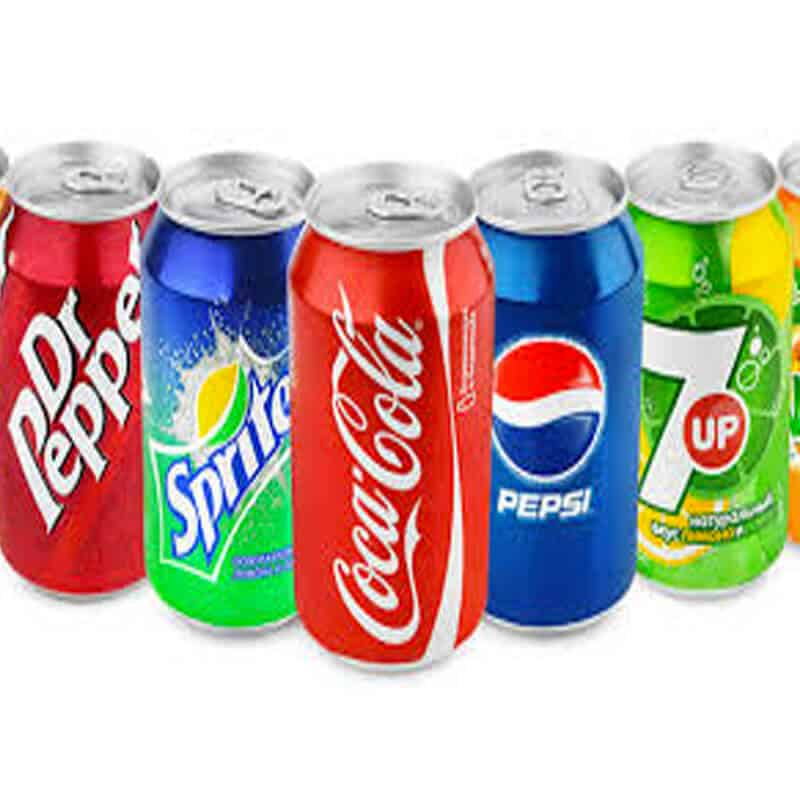
\includegraphics[scale=0.15]{sodas.jpg}
    \end{center}
    \uncover<2->{Quelle est la meilleure?}
  \end{frame}

  \begin{frame}{Les boissons}
    Qu'est-ce que ce sont? \\
    \underline{\uncover<2->{des vins: un vin blanc, un vin rosé et un vin rouge}}
    \begin{center}
      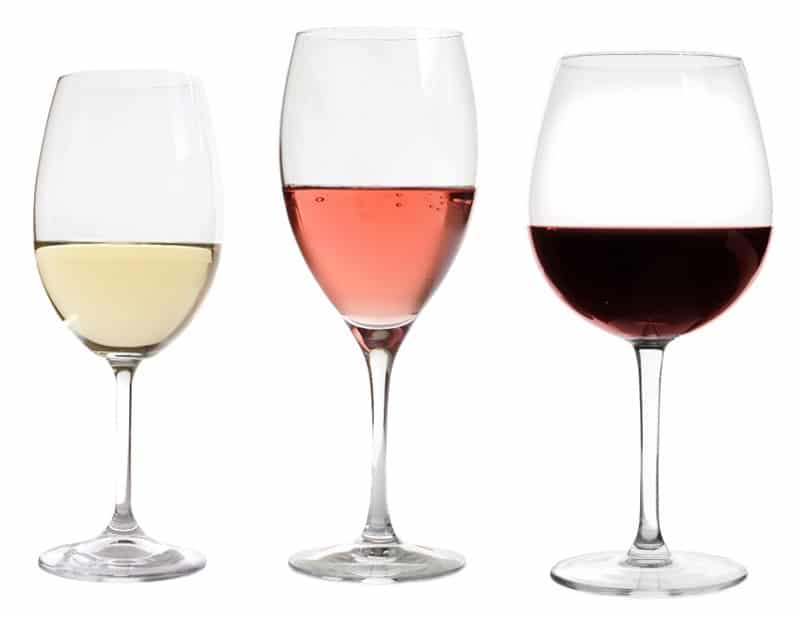
\includegraphics[scale=0.2]{vins.jpg}
    \end{center}
    \uncover<2->{Quel est le meilleur?}
  \end{frame}

  \begin{frame}{Les boissons}
    Qu'est-ce que ce sont? \\
    \underline{\uncover<2->{des jus (d'orange, de tomate, d'ananas, de pomme et de carotte)}}
    \begin{center}
      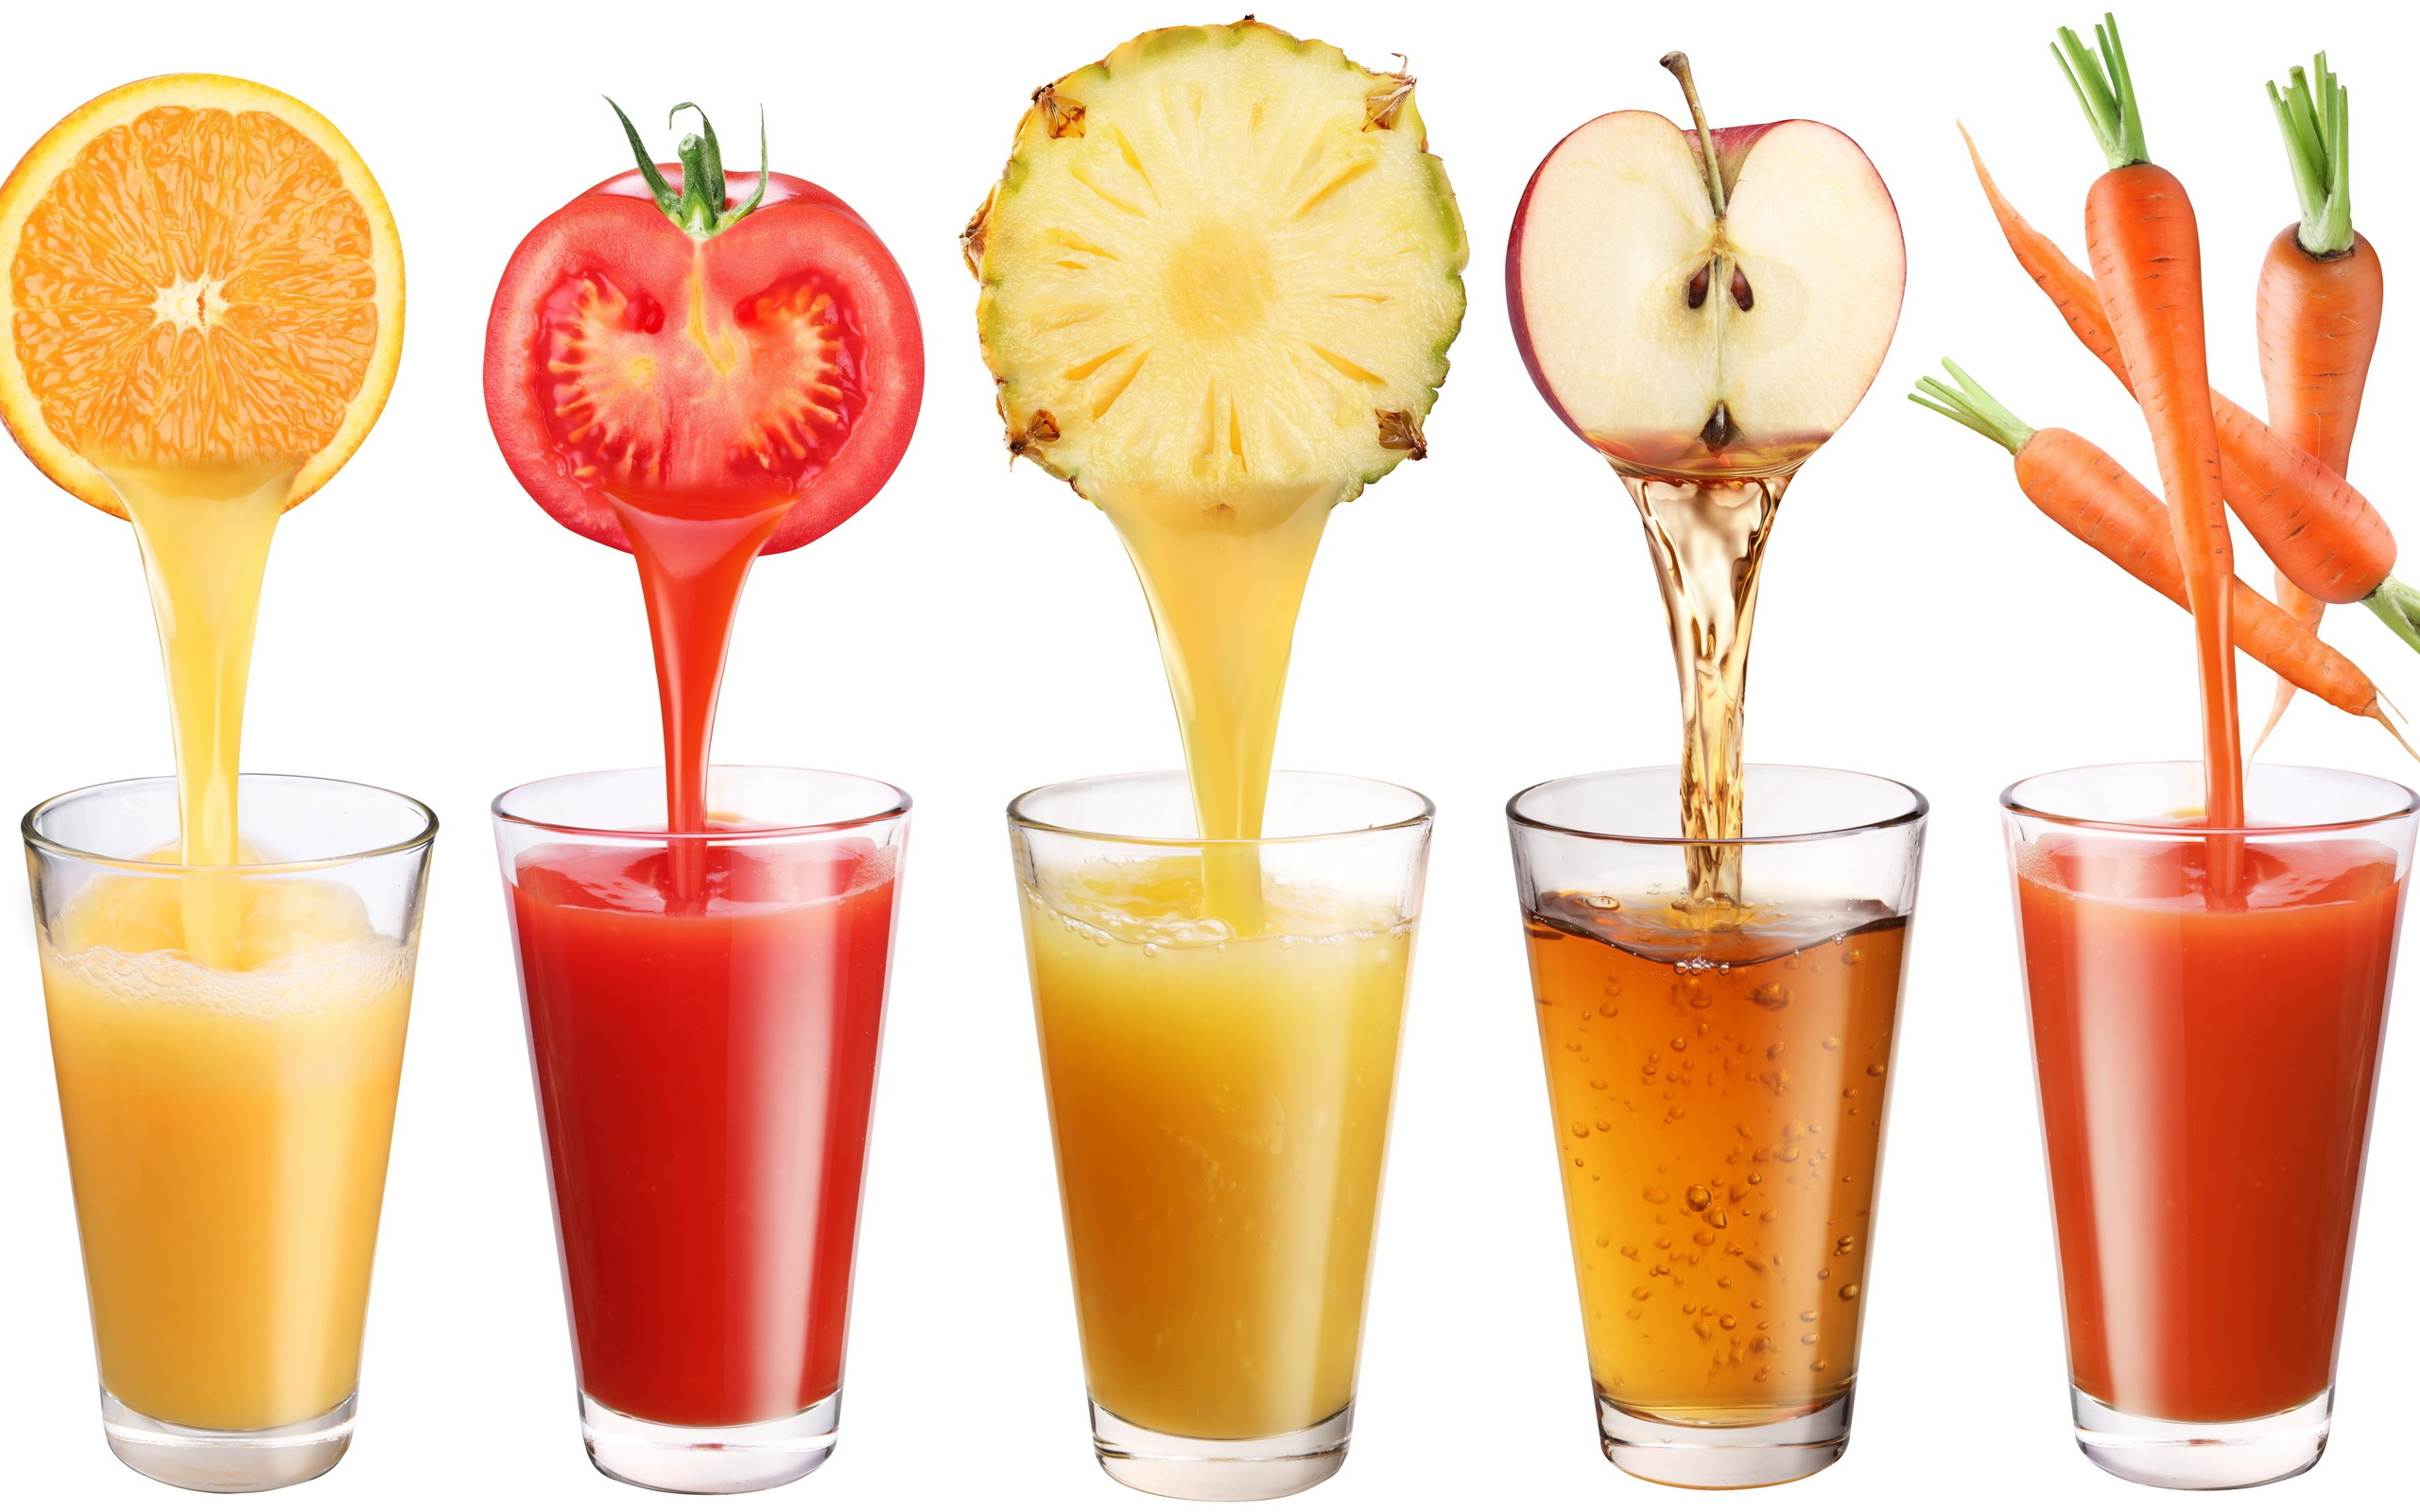
\includegraphics[scale=0.3]{jus.jpg}
    \end{center}
    \uncover<2->{Quel est le meilleur?}
  \end{frame}

  \begin{frame}{Les boissons}
    Qu'est-ce que ce sont? \underline{\uncover<2->{des eaux minérales}}
    \begin{center}
      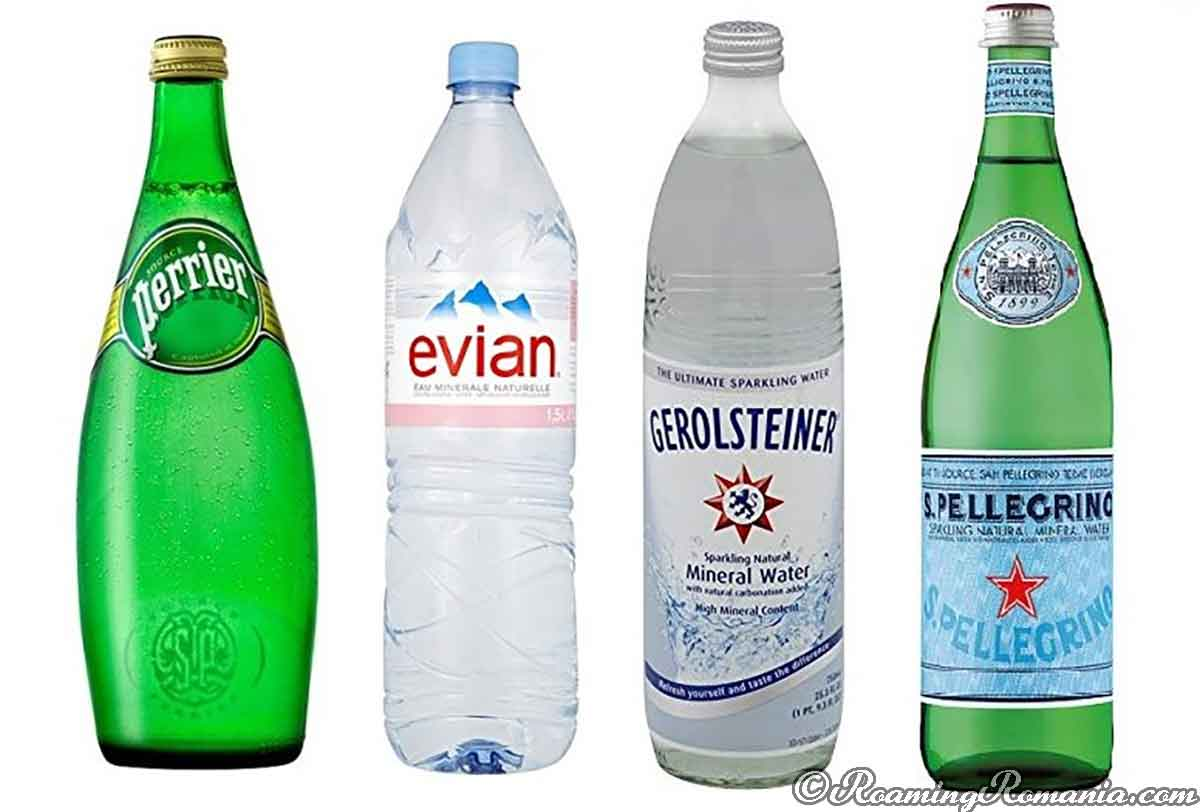
\includegraphics[scale=0.15]{eaux.jpg}
    \end{center}
    \uncover<2->{Quelle est la meilleure?}
  \end{frame}

  \begin{frame}{Les boissons}
    Qu'est-ce que ce sont? \underline{\uncover<2->{des bières}}
    \begin{center}
      \includegraphics[scale=0.35]{bières.jpg}
    \end{center}
    \uncover<2->{Quelle est la meilleure?}
  \end{frame}

  \begin{frame}{}
    \begin{center}
      \Large Quiz
    \end{center}
  \end{frame}

  \begin{frame}{Les voyelles nasalisées}
    Quel mot entendez-vous? <non-nasalisée> vs <nasalisée>
    \begin{columns}[t]
      \column{0.5\textwidth}
        \begin{enumerate}
          \item sept sainte
          \item beau bon
          \item gras grand
          \item ça cent
        \end{enumerate}
      \column{0.5\textwidth}
        \begin{enumerate}
          \setcounter{enumi}{4}
          \item sec cinq
          \item peau pont
          \item chat chant
        \end{enumerate}
    \end{columns}
    \vspace{0.5cm}
    D'habitude, on indique la nasalisation avec un \orth{n} suivi d'une autre consonne. \\
    \tinygloss{Typically, nasalization is indicated with an \orth{n} followed by another consonant.}
  \end{frame}

  \begin{frame}{Comprendre et apprendre}
    \begin{columns}[t]
      \column{0.45\textwidth}
        {\small
        Commence avec un/e partenaire.
        Pour chaque numéro, dis si tu \alert{comprends} ou si tu veux \alert{apprendre} la chose.
        Si vous ne comprenez pas la chose, séparez-vous et trouvez des groupes où on comprend cette chose, puis continue.} \\
        \tinygloss{Start with a partner.
        For each number, say whether you \alert{understand} or want to \alert{learn} the the thing.
        If you two don't understand the thing, split up and find groups where someone does understand that thing, then continue.}
      \column{0.55\textwidth}
        \scriptsize
        \begin{description}
          \item[\textbf{Modèle:}] \emph{la mode}
          \item[E1:] Moi, je ne comprends pas la mode, mais je veux apprendre. Est-ce que tu comprends la mode?
          \item[E2:] Oui, je comprends la mode.
        \end{description}
        \begin{columns}[t]
          \column{0.5\linewidth}
            \begin{enumerate}
              \item le verbe \lexi{mettre}
              \item les couleurs
              \item la littérature
              \item les adverbes
              \item le football américain
              \item la musique
              \item les chiens
              \item la mode
            \end{enumerate}
          \column{0.5\linewidth}
            \begin{enumerate}
              \setcounter{enumi}{8}
              \item le dessin
              \item l'espagnol
              \item la chimie
              \item les chats
              \item le jardinage
              \item les films
              \item le rugby
              \item l'astronomie
            \end{enumerate}
        \end{columns}
    \end{columns}
  \end{frame}

  \begin{frame}{}
    \begin{center}
      \Large Questions?
    \end{center}
  \end{frame}
\end{document}
